\chapter{Database diagram and queries used}

\begin{figure}[!htbp]
    \centering
    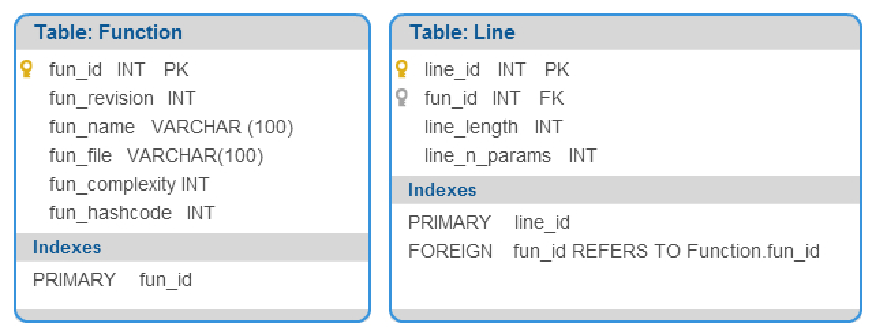
\includegraphics[width=\textwidth,keepaspectratio]{figure/methods/database_diagram.pdf}
    \caption{Database diagram generated by the automatic parsing tool}
    \label{fig:database_diagram}
\end{figure}

\begin{listing}[htbp]
\begin{minted}{sql}
SELECT 
    FUN_REVISION AS REVISION,
    AVG(CAST(FUN_COMPLEXITY AS DOUBLE)) AS AVG
FROM 
    FUNCTION 
GROUP BY 
    FUN_REVISION 
ORDER BY 
    FUN_REVISION
\end{minted}
\caption{Query to calculate the revision based average complexity}
\label{listing:avg_complexity_query}
\end{listing}

\begin{listing}[htbp]
\begin{minted}{sql}
SELECT
    CAST(s2.count as DOUBLE)/s1.count*100 as percentage,
    s1.revision   as revision
FROM
	(
		SELECT 
		    f.fun_revision as revision,
		    count(l.*) as count
		FROM
		    function as f join line as l on f.fun_id = l.fun_id
		GROUP BY
			f.fun_revision
		ORDER BY  
			f.fun_revision
	) as s1 join (
		SELECT 
		    f.fun_revision as revision,
		    count(l.*) as count
		FROM
		    function as f join line as l on f.fun_id = l.fun_id
		WHERE 
			l.line_length > 80
		GROUP BY  
			f.fun_revision
		ORDER BY  
			f.fun_revision
	) as s2 on s1.revision = s2.revision
\end{minted}
\caption{Query to calculate the percentage of complex statements on a revision basis}
\label{listing:percentage_complex_statements}
\end{listing}


\begin{listing}[htbp]
\begin{minted}{sql}
SELECT
	avg(cast(res.n_lines as double)) as avg,
	res.revision as revision
FROM
	(SELECT
		l.fun_id as id, 
		count(l.*) as n_lines, 
		f.fun_revision as revision
	FROM
		function as f join line as l on f.fun_id = l.fun_id
	GROUP BY
	        f.fun_id,
		f.fun_revision
	ORDER BY
		f.fun_revision,
		f.fun_id
	) as res
GROUP BY 
	res.revision
ORDER BY
	res.revision
\end{minted}
\caption{Query to calculate the average function length (LOC) on a commit basis}
\label{listing:avg_length_query}
\end{listing}